% !TeX spellcheck = en_US
\subsection{Weighted Histogram Analysis Method\label{Sec:FEM:WHAM}}
The weighted histogram analysis method is a generalization of the histogram method developed by Ferrenberg and Swendsen.\cite{FerrenbergPRL1989}
\subsubsection{Weighted Histogram Analysis Method for Parallel Tempering\label{Sec:FEM:WHAM_REMD}}
The following derivation quite follows Ref.~\cite{ChoderaJCTC2007}.
One of the central quantities in statistical mechanics is configurational integral $Z$, which in textbook is often written as
\begin{equation}
Z=\int \exp{(-\beta U(\mathbf{R}))}\diff\mathbf{R}.
\end{equation}
This is an integral in coordinate space. It also can be written as an integral in energy space
\begin{equation}
Z=\int \Omega(U)\exp{(-\beta U)}\diff U,
\end{equation}
where $\Omega(U)$ is density of states and $\Omega(U)\Delta U$ is the number of states in the region $U-\Delta U/2<U<U+\Delta U/2$. Accordingly, the statistical expectation of an operator $\mathbf{A}$ can be calculated by
\begin{equation}
\langle \mathbf{A}\rangle=\frac {\int \mathbf{A}(U)\Omega(U)\exp{(-\beta U)}\diff U}{\int \Omega(U)\exp{(-\beta U)}\diff U},
\end{equation}
where
\begin{equation}
\mathbf{A}(U^\prime)=\frac{\int \delta (U(\mathbf{R})-U^\prime)\mathbf{A}(\mathbf{R})\diff \mathbf{R}}{\int \delta (U(\mathbf{R})-U^\prime)\diff\mathbf{R}},
\end{equation}
is the average of $\mathbf{A}$ over all the samples with an energy $U^\prime$. Therefore, the core objective is to calculate $\Omega(U)$.

Suppose we have one trajectory with $N$ snapshots denoted as $\{\mathbf{R}_n\}$. We then discretize the energy space into $M$ bins with width $\Delta U$, and count the number of snapshots into each bin. For convenience, we define $\psi_m(U)$ as
\begin{equation}
	\psi_m(U)= 
	\left\{ 
	\begin{array}{rl} 
	1 & \text{if }U\in \left[ U_m-\Delta U/2, U_m+\Delta U/2\right)\\ 
	0 & \text{otherwise}\\  
	\end{array} 
	\right. 
\end{equation}
Then the histogram for the $m$th energy bin is
\begin{equation}
	H_{m}=\sum\limits_{n=1}^{N}\psi_{m}(U(\mathbf{R}_n))=N\cdot \frac 1 N\sum\limits_{n=1}^{N}\psi_{m}(U(\mathbf{R}_n))=N\cdot\left<\psi_m\right>,
\end{equation}
with variances (see Appendix~\ref{chapter:Appendix:Uncertainty})
\begin{align}
	\delta^2 H_m=&N^2\delta^2(\left<\psi_m\right>)\notag\\
	            =&g_m N\left(\left<{\psi_m}^2\right>-\left<\psi_m\right>^2\right)\notag\\
	            =&g_m N\left(\left<\psi_m\right>-\left<\psi_m\right>^2\right)\notag\\
	            =&g_m H_m\left(1-\frac{H_m}{N}\right).
\end{align}

A sample histogram in 2D space is shown in Fig.~\ref{Fig:FEM:WHAM:histogram}.
\begin{figure}[htbp]
	\centering
    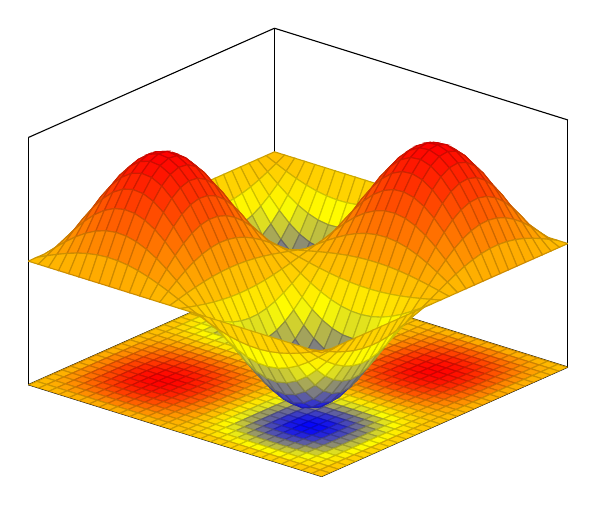
\begin{tikzpicture}
        \begin{axis}[xtick=\empty, ytick=\empty, ztick=\empty, minor tick num=0,view/h=40]
        
          \addplot3[surf,
          mesh/color input=colormap,
          colormap/hot,
          domain=-180:180, y domain=-180:180,
          point meta={sin(x)*sin(y)},
          point meta rel=per plot,
          point meta min=-1.0, point meta max=1.0,
          shader=faceted,
          update limits=false,
          on layer=axis background,
          samples=30
          ] {-1.2};
          \addplot3[surf, shader=faceted, domain=-180:180, y domain=-180:180, samples=30] 
          {sin(x)*sin(y)};
%         \addplot3[surf, shader=faceted, domain=-180:180, y domain=-180:180, samples=20, color=black, point meta rel=per plot, point meta={sin(x)*sin(y)} ] {-1.0};

        \end{axis}
    \end{tikzpicture}
    \caption{A sample histogram in 2D space, for instance potential energy and a reaction coordinate $\xi$.}\label{Fig:FEM:WHAM:histogram}
\end{figure}
%\begin{figure}[htbp]
%	\centering
%	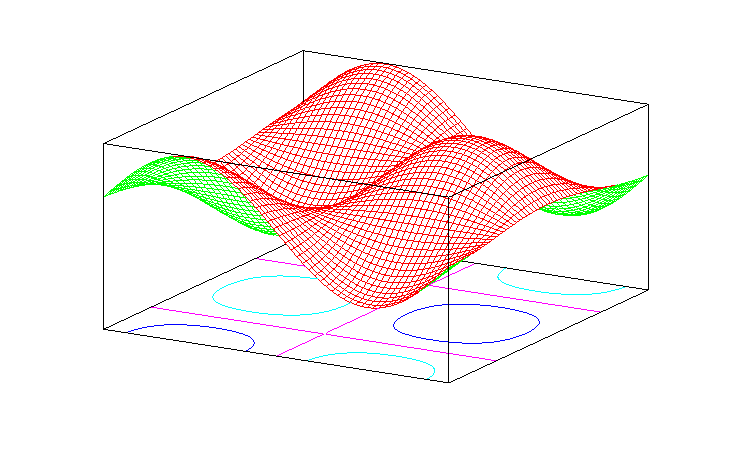
\includegraphics[width=0.8\textwidth]{figures/histogram.pdf}\\
%	\caption{A sample histogram in 2D space, for instance potential energy and a reaction coordinate $\xi$.}\label{Fig:FEM:WHAM:histogram}
%\end{figure}

The ratio of the histogram $H_m$ to the total number of snapshots $N$ divided by the bin width $\Delta U$ can be approximately taken as the probability of states in this bin, i.e.,
\begin{equation}
	\frac{\Omega_m\exp{(-\beta U_m)}}{Z}\approx\frac{H_m}{N\Delta U}.
\end{equation}
Therefore,
\begin{align}
	\Omega_m=&\frac{1}{\Delta U}\cdot\frac{H_m}{N}\cdot\frac{Z(\beta)}{\exp{(-\beta U_m)}}\notag\\
	        =&\frac{H_m}{N\Delta U\exp{\left[f-\beta U_m\right]}},
	\label{Eq:FEM:WHAM:DoSsingle}
\end{align}
and variances
\begin{equation}
	\delta^2\Omega_m=\frac{\delta^2 H_m}{\left(N\Delta U\exp{\left[f-\beta U_m\right]}\right)^2},
\end{equation}
in which we have defined a dimensionless free energy $f=-\ln{Z(\beta)}$.

Practically, we may run multiple ($K$) trajectories using, for example, replica exchange molecular dynamics simulations. For each trajectory (index $k$), we have unique estimators for the histogram $H_{mk}$, the density of states $\Omega_{mk}$ and their variances $\delta^2 H_{mk}$ and $\delta^2\Omega_{mk}$ being
\begin{equation}
	H_{mk}=\sum\limits_{n=1}^{N_k}\psi_{m}(U(\mathbf{R}_{kn})),
\end{equation}
\begin{equation}
	\delta^2 H_{mk}=g_{mk}H_{mk}\left(1-\frac{H_{mk}}{N_k}\right),
\end{equation}
\begin{align}
	\Omega_{mk}=\frac{H_{mk}}{N_k\Delta U\exp{\left[f_k-\beta_kU_{m}\right]}},
	\label{Eq:FEM:WHAM:Omega_mk}
\end{align}
and
\begin{equation}
	\delta^2\Omega_{mk}=\frac{\delta^2 H_{mk}}{\left(N_k\Delta U\exp{\left[f_k-\beta_kU_{m}\right]}\right)^2},
\end{equation}
The optimum estimator of the density of states from all the simulations is
\begin{equation}
	\Omega_m=\frac{\sum\limits_{k=1}^K\left[\delta^2\Omega_{mk}\right]^{-1}\Omega_{mk}}{\sum\limits_{k=1}^K\left[\delta^2\Omega_{mk}\right]^{-1}},
	\label{Eq:FEM:WHAM:optimumOmega}
\end{equation}
which is the weighted average of density of states of all the trajectories with the weight reversely proportional to the variances (see Appendix~\ref{chapter:Appendix:Mean}).

To make the expression simpler, here we take some approximations. First, normally the energy space is split into a large number of bins. The histogram in each bin is much smaller than the total number of snapshots, i.e. $H_{mk}\ll N_k$. With this approximation, we have
\begin{align}
	\delta^2 H_{mk}\approx g_{mk}H_{mk}.
\end{align}
The expectation of $H_{mk}$ can be related to the optimum estimator of the density of states, i.e.
\begin{equation}
	\overline{H_{mk}}=N_k\Delta U\Omega_m\exp{(f_k-\beta_kU_m)}.
\end{equation}
Then we have
\begin{equation}
    \delta^2H_{mk}=g_{mk}N_k\Delta U\Omega_m\exp{(f_k-\beta_kU_m)}
    \label{EQ:FEM:WHAM:delta2H_mk}
\end{equation}
and
\begin{equation}
\delta^2\Omega_{mk}=\frac{\Omega_m}{{g_{mk}}^{-1}N_k\Delta U\exp{(f_k-\beta_kU_m)}}.
\label{Eq:FEM:WHAM:delta2Omega_mk}
\end{equation}

Taking Eq.~\ref{Eq:FEM:WHAM:Omega_mk} and Eq.~\ref{Eq:FEM:WHAM:delta2Omega_mk} into Eq.~\ref{Eq:FEM:WHAM:optimumOmega}, we find
\begin{equation}
\Omega_m=\frac{\sum\limits_{k=1}^{K}{g_{mk}}^{-1}H_{mk}}{\sum\limits_{k=1}^{K}{g_{mk}}^{-1}N_k\Delta U\exp{(f_k-\beta_kU_m)}},
\label{Eq:FEM:WHAM:Omega_iteration}
\end{equation}
in which
\begin{equation}
f_k=-\ln \int \Omega(U)\exp{(-\beta_k U)}\diff U=-\ln\sum\limits_{m=1}^M\Omega_m\Delta U\exp{(-\beta_kU_m)}.
\label{Eq:FEM:WHAM:f_k_iteration}
\end{equation}
Obviously, Eq.~\ref{Eq:FEM:WHAM:Omega_iteration} and Eq.~\ref{Eq:FEM:WHAM:f_k_iteration} must be solved iteratively.
Applying the error propagation rule to Eq.~\ref{Eq:FEM:WHAM:Omega_iteration} and using Eq.~\ref{EQ:FEM:WHAM:delta2H_mk}, the variance of $\Omega_m$ is given by
\begin{equation}
\delta^2 \Omega_m=\frac{\Omega_m}{\sum\limits_{k=1}^K{g_{mk}}^{-1}N_k\Delta U\exp{(f_k-\beta_kU_m)}}.
\end{equation}
%and the relative variance is given by
%\begin{equation}
%\frac{\delta^2\Omega_m}{\Omega_m^2}=\left[\sum\limits_{k=1}^K{g_{mk}}^{-1}H_{mk}\right]^{-1}.
%\end{equation}
Using the density of states and its variance, we can estimate the expectation of any configuration function $A(\mathbf{R})$ at any inverse temperature $\beta$
\begin{equation}
\left<A\right>_\beta\approx\frac{\sum\limits_{m=1}^M\Omega_m\Delta U\exp{(-\beta U_m)}A_m}{\sum\limits_{m=1}^M\Omega_m\Delta U\exp{(-\beta U_m)}},
\label{Eq:FEM:WHAM:A}
\end{equation}
where
\begin{equation}
A_m=\frac{\int \diff\mathbf{R}A(\mathbf{R})\psi_m(U(\mathbf{R}))}{\int \diff\mathbf{R}\psi_m(U(\mathbf{R}))}.
\end{equation}
Using histograms of bin $m$ from all the simulations and defining $H_m=\sum\limits_{k=1}^KH_{mk}$, an estimator of $A_m$ denoted as $\hat{A}_m$ can be calculated as
\begin{equation}
   \hat{A}_m={H_{m}}^{-1}\sum\limits_{k=1}^K\sum\limits_{n=1}^{N_k}\psi_m(U(\mathbf{R}_{kn}))A(\mathbf{R}_{kn}).
   \label{Eq:FEM:WHAM:A_m}
\end{equation}
Taking Eq.~\ref{Eq:FEM:WHAM:A_m} into Eq.~\ref{Eq:FEM:WHAM:A}, we obtain an estimator of $\hat{A}(\beta)$
\begin{align}
\hat{A}(\beta)=&\frac{\sum\limits_{m=1}^M\Omega_m\Delta U\exp{(-\beta U_m)}{H_{m}}^{-1}\sum\limits_{k=1}^K\sum\limits_{n=1}^{N_k}\psi_m(U(\mathbf{R}_{kn}))A(\mathbf{R}_{kn})}{\sum\limits_{m=1}^M\Omega_m\Delta U\exp{(-\beta U_m)}}\\
              =&\frac{\sum\limits_{m=1}^M\Omega_m\Delta U\exp{(-\beta U_m)}{H_{m}}^{-1}\sum\limits_{k=1}^K\sum\limits_{n=1}^{N_k}\psi_m(U(\mathbf{R}_{kn}))A(\mathbf{R}_{kn})}{\sum\limits_{m=1}^M\Omega_m\Delta U\exp{(-\beta U_m)}{H_{m}}^{-1}\sum\limits_{k=1}^K\sum\limits_{n=1}^{N_k}\psi_m(U(\mathbf{R}_{kn}))}\\
              =&\frac{\sum\limits_{k=1}^K\sum\limits_{n=1}^{N_k}w_{kn}(\beta)A_{kn}}{\sum\limits_{k=1}^K\sum\limits_{n=1}^{N_k}w_{kn}(\beta)},
\end{align}
where the per-configuration weights $w_{kn}(\beta)$ is given by
\begin{equation}
w_{kn}(\beta)=\sum\limits_{m=1}^M{H_{m}}^{-1}\psi_m(U(\mathbf{R}_{kn}))\Omega_m\exp{(-\beta U_m)}
\end{equation}

\subsubsection{Weighted Histogram Analysis Method From Minimizing Statistical Error}
In this section, the ``traditional'' derivation method of WHAM are briefly reviewed.\cite{SouailleCPC2001} In the WHAM, the goal is to get an optimal unbiased probability distribution $\rho_{0}(\eta)$, where $\eta$ is a series of discretized histogram bins indexed by $j=1,2,3,...,M$ along a certain reaction coordinate. WHAM can be used to analyze the Umbrella Sampling (US) simulations, where a set of simulations indexed by $i$ or $k=1,2,3,...,S$ are performed with a series of biasing potentials added on the reaction coordinate $\eta$. To consider a reference molecular system with the potential energy $U_{0}(\textbf{x})$, where $\textbf{x}$ is the set of atomic coordinates. The reaction coordinate $\eta$ is a function of the atomic coordinates, i.e. $\eta(\textbf{x})$. To suppose that the $i$th molecular simulation has been performed using potential energy function
\begin{equation}
U_{i}^{(b)}(\eta) = U_{0}(\textbf{x}) + W_{i}(\eta(\textbf{x})),
\label{Eq:FEM:WHAM:biasmd}
\end{equation}
where $W_{i}(\eta(\textbf{x}))$ is the biasing potential added on the reaction coordinate $\eta$, e.g. $W_{i}(\eta)=\frac{1}{2}k_{i}(\eta-\eta_{i})^2$ in a harmonic form. From these simulations a set of normalized biased probability distributions ${\rho_{i}^{(b)}(\eta)}$ can be obtained.
\begin{equation}
\rho_{i}^{(b)}(\eta) = \frac{e^{-\beta U_{i}^{(b)}(\eta)}}{Q_{i}^{(b)}},
\label{Eq:FEM:WHAM:bias}
\end{equation}
where $Q_{i}^{(b)}=\int e^{-\beta U_{i}^{(b)}(\eta)} \diff\eta = e^{-\beta f_{i}^{(b)}}$ and $f_{i}^{(b)}$ is the biased free energy.
The corresponding unnormalized unbiased probability distribution $\rho_{i}^{(u)}(\eta)$ from the $i$th simulation is defined as, 
\begin{align}
\rho_{i}^{(u)}(\eta) = e^{\beta[W_{i}(\eta)-f_{i}^{(b)}]}\rho_{i}^{(b)}(\eta)
\label{Eq:FEM:WHAM:unbias}
\end{align}
In the following, the free energy $f_{i}^{(b)}$ is assumed to be known. 
It has been shown that in the WHAM method, the total normalized unbiased probability distribution $\rho_{0}(\eta)$ can be obtained by a linear $\eta$-dependent combination of the unbiased histograms $\rho_{i}^{(u)}(\eta)$ 
\begin{equation}
\rho_{0}(\eta)=C\sum_{i=1}^{S}p_{i}(\eta)\rho_{i}^{(u)}(\eta),
\label{Eq:FEM:WHAM:unbias0}
\end{equation}  
where $C$ is the normalization factor. $p_i$ is the weight to be optimized, which is under a constraint that
\begin{equation}
\sum_{i=1}^{S}p_{i}(\eta)=1.
\label{Eq:FEM:WHAM:p1}
\end{equation}
These weights are chosen so as to minimize the statistical error made on the total unbiased probability distribution $\rho_{0}(\eta)$, that is, for any given value of $\eta$,
\begin{equation}
\frac{\partial(\sigma^2[\rho_{0}(\eta)])}{\partial p_{i}(\eta)}=0.
\label{Eq:FEM:WHAM:partialp}
\end{equation} 
It can be easily found that $\rho_{0}(\eta)$ satisfy
\begin{align}
\rho_{0}(\eta) = & C\sum_{i=1}^{S}\frac{N_{i}e^{-\beta[W_{i}(\eta)-f_{i}^{(b)}]}}{\sum_{k=1}^{S}N_{k}e^{-\beta[W_{k}(\eta)-f_{k}^{(b)}]}}\rho_{i}^{(u)}(\eta) \notag\\
= & C\sum_{i=1}^{S}\frac{N_{i}}{\sum_{k=1}^{S}N_{k}e^{-\beta[W_{k}(\eta)-f_{k}^{(b)}]}}\rho_{i}^{(b)}(\eta) \notag\\
= & C\frac{\sum_{i=1}^{S}N_{i}\rho_{i}^{(b)}(\eta)}{\sum_{k=1}^{S}N_{k}e^{-\beta[W_{k}(\eta)-f_{k}^{(b)}]}},
\label{Eq:FEM:WHAM:unbias02}
\end{align} 
where $\rho_{i}^{(b)}(\eta)$ can be written as a $\delta$ function,
\begin{equation}
\rho_{i}^{(b)}(\eta) \equiv \frac{1}{N_{i}} \sum_{l=1}^{N_{i}} \delta {(\eta-\eta_{i,l})},
\label{Eq:FEM:WHAM:delta01}
\end{equation} 
where $\eta_{i,l}$ is the reaction coordinates of the $l$th configuration in the $i$th biased simulation .

Until now, the treatment assumes that the free energy parameters ${f_{i}^{(b)}}$ are known. In fact, these parameters can be obtained self-consistently. Indeed, the definition of the free energy $f_{i}^{(b)}$ is,
\begin{align}
e^{-\beta f_{i}^{(b)}}=&\int e^{-\beta U_{i}^{(b)}(\eta) } \diff\eta \notag\\
=&\int \rho_{0}(\eta) e^{-\beta W_{i}(\eta)} \diff\eta \notag\\
=&C \int \frac{\sum_{i=1}^{S}N_{i}\rho_{i}^{(b)}(\eta)}{\sum_{k=1}^{S}N_{k}e^{-\beta[W_{k}(\eta)-f_{k}^{(b)}]}}e^{-\beta W_{i}(\eta)}  \diff\eta
\label{Eq:FEM:WHAM:fi01}
\end{align} 
The set of parameters ${f_{i}^{(b)}}$ appear on both sides of Eq.~\ref{Eq:FEM:WHAM:fi01}, which must be solved iteratively with an initial guess of ${f_{i}^{(b)}}$ until convergence is reached. The unbiased free energy corresponding to the histogram can be calculated by
\begin{equation}
f_{0}(\eta)=-\beta^{-1}\ln \rho_{0}(\eta) 
\label{Eq:FEM:WHAM:f0}
\end{equation}
with $W$ in Eq.~\ref{Eq:FEM:WHAM:fi01} being 0.
The constant $C$ in Eq.~\ref{Eq:FEM:WHAM:unbias02} is irrelevant, which only causes a constant shift to the free energy profiles. To get rid of it, one may subtract the offset constant $f_{0}(\eta_{1})$ from all the $f_{0}(\eta_{j})$.  

\subsubsection{Weighted Histogram Analysis Method From Maximum Likelihood}
The following derivation quite follows Ref.~\cite{GallicchioJPCB2005}, in which maximum likelihood principle is utilized. 
Suppose we have performed $K$ simulations, each at a different inverse temperature $\beta_k$ and possibly with different biasing potential $w_k(\mathbf{R})$.
We then discretize the 2D plane spanned by the coordinate and unbiased potential energy into bins, each characterized by ${\mathbf{R}_j}$ and ${E_h}$. To make the following derivation cleaner, we map the 2D bins to one dimensional series with index $l, l=1,\dots,L$. Next, we construct histograms for bins using all the samples from the simulations. The probability of finding the system in bin $l$ during the $k$th simulation can be written as
\begin{equation}
p_{k,l}=f_kc_{k,l}p_l^0,
\label{Eq:FEM:WHAM:unbiasingProb}
\end{equation}
in which $p_l^0$ is the (simulation-independent) unbiased probability,
\begin{align}
c_{k,l}=&\exp{\left[-\beta_k\left(E_l+w_{k,l}\right)+\beta_0E_l\right]}\notag\\
=&\exp{\left[-\left(\beta_k-\beta_0\right)E_l\right]}\exp{\left(-\beta_kw_{k,l}\right)}
\end{align}
is the bias factor, $E_l$ is the unbiased energy of bin $l$, $f_k={\left\{\sum\limits_lc_{k,l}p_l^0\right\}}^{-1}$ is the normalization factor. If we expand the expressions for $c_{k,l}$ and $p_l^0$, we find
\begin{align}
	f_k\approx&\left(\sum\limits_l \exp{\left[-\beta_k\left(E_l+w_{k,l}\right)+\beta_0E_l\right]} \frac{\exp{(-\beta_0 E_l)}}{\sum\limits_j\exp{(-\beta_0 E_j)}}\right)^{-1}\notag\\
	   =&\left(\frac{\sum\limits_l\exp{\left[-\beta_k(E_l+w_{k,l})\right]}}{\sum\limits_j\exp{(-\beta_0 E_j)}}\right)^{-1}\notag\\
	   \approx&\frac{Z_0}{Z_k},
\end{align}
which is approximately the ratio of two configurational integrals.

It is worth emphasizing that the biasing potential can be multiple dimensional as, for instance, in a two-dimensional umbrella sampling.
If the biasing is only in temperature-space as in replica exchange molecular dynamics
\begin{equation}
c_{k,l}=\exp{\left[-\left(\beta_k-\beta_0\right)E_l\right]},
\end{equation} 
while if the biasing is only in potential energy as in umbrella sampling
\begin{equation}
c_{k,l}=\exp{\left(-\beta_0w_{k,l}\right)}.
\end{equation}

If we assume that each count in each histogram is independent, then the likelihood of observing the $k$th histogram distribution is given by the multinomial distribution
\begin{align}
P(n_{k,1},n_{k,2},\dots,n_{k,L}|p_{k,1},p_{k,2},\dots,p_{k,L})=\notag\\
\frac{\left(\sum\limits_l n_{k,l}\right)!}{\prod\limits_l n_{k,l}!}\prod\limits_{l=1}^L\left(p_{k,l}\right)^{n_{k,l}}\propto\prod\limits_{l=1}^{L}\left(f_kc_{k,l}p_l^0\right)^{n_{k,l}}.
\end{align}
For all $K$ simulations, the likelihood is the product of multinomial
\begin{align}
P(n_{1,1},\dots,n_{1,L};\dots;n_{K,1},\dots,n_{K,L}|p_1^0,\dots,p_L^0)\propto\notag\\
\prod\limits_{k=1}^K\prod\limits_{l=1}^{L}\left(f_kc_{k,l}p_l^0\right)^{n_{k,l}},
\label{Eq:FEM:WHAM:totalProb}
\end{align}
where the likelihood is conditional only on the unbiased probabilities $p_l^0$, since the bias factors $c_{k,l}$ are known parameters, and the normalization constants $f_k$ are known conditional on $p_l^0$. The maximum likelihood estimate of the unbiased probabilities can be found by maximizing $P$ in Eq.~\ref{Eq:FEM:WHAM:totalProb} with respect to $p_1^0,\dots,p_L^0$ and are given by solutions of the simultaneous nonlinear equations
\begin{equation}
p_l^0=\frac{\sum\limits_{k=1}^K n_{k,l}}{\sum\limits_{k=1}^K N_kf_kc_{k,l}}\, (\text{for each }l)
\end{equation}
and
\begin{equation}
f_k={\left\{\sum\limits_lc_{k,l}p_l^0\right\}}^{-1},
\end{equation}
where $N_k$ is the total number of counts in the $k$th histogram. This is equivalent to the maximum \textit{a posteriori} (MAP) estimation with a uniform \textit{prior} probability for $p_l^0$\cite{FergusonJCC2017}.

\subsubsection{Binless Weighted Histogram Analysis Method\label{Sec:FEM:WHAM_BINLESS}}
The following derivation quite follows Ref.~\cite{TanJCP2012}.
Let us start with the definition of a generalized energy function $u$ and its corresponding coefficient $\theta$. For instance, for canonical ensemble, $u=U(x)$ is the potential energy function, and $\theta=\beta$ is the inverse temperature. For isothermal grand-canonical ensemble, $u=(U(x),N)$, and $\theta=(\beta,\beta\mu)$, in which $N$ is the number of particles and $\mu$ is the chemical potential. For temperature replica exchange molecular dynamics, $u=U(x)$ and $\theta_k=\beta_k$ for the $k$th replica. For umbrella sampling, $u=(U_0(x),\omega_1(x),\omega_2(x),\dots,\omega_d(x))$, where $U_0(x)$ is the unbiased Hamiltonian and $\omega_k(x)$ is the biasing potential in window $k$. Correspondingly, $\theta_k=(\beta,0,\dots,0,\beta,0,\dots,0)$, in which all the elements are zero except for the first and the $(k+1)$th element.

Assume that simulations are conducted at $m$ coefficient vectors $\theta_r\, (r=1,\dots,m)$ and with the same energy vector $u(x)$. (Note that in this notation the dimensionality, $d$, of the $\theta$ and $u$ vectors and the number of simulations, $m$, are, in general, distinct. For instance, for temperature replica exchange molecular dynamics as shown above, $d=1$, while $m$ is the number of replicas.) Denoted by $\{x_{ji}: i=1,\dots,n_j\}$ the set of configurations of size $n_j$ from the the $j$th simulation, and denoted by $u_{ji}=u(x_{ji})$ the corresponding generalized energy vectors. The total sample size is $n=\sum_{j=1}^m n_j$. Now, consider a generalized ensemble whose Boltzmann probability density function is
\begin{equation}
\frac{1}{Z_\theta}e^{-\theta^\mathrm{T}u(x)},
\end{equation}
where
\begin{equation}
Z_\theta=\int e^{-\theta^\mathrm{T}u(x)}\diff{x}
\end{equation}
is the generalized configurational integral in physics or the normalization constant in statistics, and the superscript $\mathrm{T}$ is the transpose operator. The induced probability density function of $u(x)$ at $\theta$ is
\begin{equation}
    \frac{1}{Z_\theta}\Omega(u)e^{-\theta^\mathrm{T}u},
\end{equation}
where $\Omega(u)$, formally defined as
\begin{equation}
    \Omega(u)=\int \delta(u(x)-u)\diff x,
\end{equation}
is a generalized density of states, which does not depend on $\theta$. The generalized configurational integral can also be determined from $\Omega(u)$ as
\begin{equation}
    Z_\theta=\int \Omega(u)e^{-\theta^\mathrm{T}u}\diff u.
\end{equation}
As we have shown that the WHAM method involves constructing a histogram, $H_r(u)$, from each sample $\{u_{ri}:\, i=1,\dots,n_r\}$, which $H_r(u)$ indicates the number of observations falling into a bin about $u$, for example, an interval or a rectangle if $u(x)$ is one or two-dimensional. Then $\Omega(u)$ is estimated by
\begin{equation}
    \hat{\Omega}(u)\Delta u=\frac{\sum_{r=1}^m H_r(u)}{\sum_{r=1}^m n_r\hat{Z}_{\theta_r}^{-1}e^{-\theta_r^\mathrm{T}u}},
    \label{Eq:FEM:WHAM:ConfIntinEner}
\end{equation}
where the configurational integrals ($Z_{\theta_1},\dots,Z_{\theta_m}$) are defined by self-consistency according to Eq.~\ref{Eq:FEM:WHAM:ConfIntinEner}
\begin{equation}
    \hat{Z}_{\theta_k}=\sum_{u}\frac{\sum_{r=1}^m H_r(u)}{\sum_{r=1}^m n_r\hat{Z}_{\theta_r}^{-1}e^{(\theta_k-\theta_r)^\mathrm{T}u}}\quad (k=1,\dots,m),
    \label{Eq:FEM:WHAM:binnedZ}
\end{equation}
where the summation $\sum_u$ is taken over all possible bins centered at $u$ of size $\Delta u$. Also, the configurational integral $Z_\theta$ at any other parameter value is estimated by
\begin{equation}
    \hat{Z}_\theta=\sum_{u}\frac{\sum_{r=1}^m H_r(u)}{\sum_{r=1}^m n_r\hat{Z}_{\theta_r}^{-1}e^{(\theta-\theta_r)^\mathrm{T}u}}.
    \label{Eq:FEM:WHEM:binweight1}
\end{equation}
We can take
\begin{equation}
    \frac{1}{\hat{Z}_\theta}\frac{\sum_{r=1}^m H_r(u)}{\sum_{r=1}^m n_r\hat{Z}_{\theta_r}^{-1}e^{(\theta-\theta_r)^\mathrm{T}u}}
    \label{Eq:FEM:WHEM:binweight2}
\end{equation}
as the weight of bin $u$ under condition $\theta$.

Now, let $h(u)$ be a function of $u$, and denoted by $\langle h\rangle_\theta$ the expectation of $h(u)$. The WHAM estimate $\hat{h}_\theta$ for $\langle h\rangle_\theta$ is
\begin{equation}
    \hat{h}_\theta=\frac{1}{\hat{Z}_\theta}\sum_u h(u) \frac{\sum_{r=1}^m H_r(u)}{\sum_{r=1}^m n_r\hat{Z}_{\theta_r}^{-1}e^{(\theta-\theta_r)^\mathrm{T}u}}.
    \label{Eq:FEM:WHAM:WHAMhu}
\end{equation}
It is interesting to note that the summation over bins in Eq.~\ref{Eq:FEM:WHAM:WHAMhu} can be equivalently expressed in terms of a weighted average over observations
\begin{equation}
    \hat{h}_{\theta}=\sum_{ji}h(u_{ji}^b)F_{ji}(\theta),
    \label{Eq:FEM:WHAM:WHAMhu2}
\end{equation}
where $u_{ji}^b$ is a representative generalized energy of the bin containing $u_{ji}$, $F_{ji}$ is the ``WHAM weight'' of $u_{ji}$ that, by comparing Eqs.~\ref{Eq:FEM:WHAM:WHAMhu} and \ref{Eq:FEM:WHAM:WHAMhu2}, is defined as
\begin{equation}
    F_{ji}(\theta)=\frac{\hat{Z}_\theta^{-1}}{\sum_{r=1}^mn_r\hat{Z}_{\theta_r}^{-1}e^{(\theta-\theta_r)^\mathrm{T}u_{ji}^b}}=\frac{1}{\hat{Z}_\theta}e^{-\theta^Tu_{ji}^b}G_{ji}
    \label{Eq:FEM:WHAM:sampleW}
\end{equation}
and 
\begin{equation}
    G_{ji}=\frac{1}{\sum_{r=1}^m n_r\hat{Z}_{\theta_r}^{-1}e^{-\theta_r^\mathrm{T}u_{ji}^b}}
\end{equation}
is the $\theta$-dependent component of the WHAM weight $F_{ji}(\theta)$ for each observation.

Equation~\ref{Eq:FEM:WHAM:WHAMhu2} states that the expectation value of any observable can be obtained by attaching a statistical weight $F_{ji}(\theta)$ to each observation $u_{ji}$ which depends on the bin to which it is assigned. An obvious simplification is to express the WHAM estimate of $\langle h\rangle_\theta$ and the WHAM weights (Eq.~\ref{Eq:FEM:WHAM:sampleW}) in terms of the actual observation $u_{ji}$ rather than their closest bin representative $u_{ji}^b$.

To understand binless WHAM, it is useful to introduce the concept of the measure $G$ defined by
\begin{equation}
    \diff G=\Omega(u)\diff u,
\end{equation}
that is, $G(A)=\int_A\Omega(u)\diff u$ for every measurable set $A$ of $u$. Informally, this equation says that for an infinitesimal bin about $u$ of size $\diff u$, the weight assigned under $G$ is $\Omega(u)\diff u$. Thereafter $G$ is called the measure of states. The probability distribution of $u(x)$, $F_\theta$, is related to $G$ as
\begin{equation}
    \diff F_\theta=\frac{1}{Z_\theta}e^{-\theta^\mathrm{T}u}\Omega(u)\diff u=\frac{1}{Z_\theta}e^{-\theta^\mathrm{T}u}\diff G,
\end{equation}
that is
\begin{equation}
    F_\theta(A)=\frac{1}{Z_\theta}\int_A e^{-\theta^\mathrm{T}u}\diff G
\end{equation}
for every measurable set $A$ of $u$. The configurational integral can then be expressed as
\begin{equation}
    Z_\theta=\int e^{-\theta^\mathrm{T}u}\diff G.
\end{equation}

The pooled data $\{u_{ji}: i=1,\dots,n_j, j=1,\dots,m\}$ can be regarded as an approximate sample from the mixture distribution, $F_\ast$, whose components are $(F_{\theta_1},\dots,F_{\theta_m})$ with proportions $(n_1/n,\dots,n_m/n)$. $F_\ast$ is related to $G$ as 
\begin{equation}
    \diff F_\ast=\left\{\sum_{r=1}^m\frac{n_r}{n}Z_{\theta_r}^{-1} e^{-\theta_r^{\mathrm{T}}u} \right\}\Omega(u)\diff u=\left\{\sum_{r=1}^m\frac{n_r}{n}Z_{\theta_r}^{-1} e^{-\theta_r^{\mathrm{T}}u} \right\}\diff G
    \label{Eq:FEM:WHAM:mixedensemble}
\end{equation}
For an infinitesimal bin about $u$ of size $\diff u$, the probability assigned under $F_\ast$ is the expression in the curly brackets times the weight assigned under $G$. Dividing both sides of Eq.~\ref{Eq:FEM:WHAM:mixedensemble} by the quantity in the curly brackets  gives
\begin{equation}
    \diff G=\left\{\sum_{r=1}^m\frac{n_r}{n}Z_{\theta_r}^{-1} e^{-\theta_r^{\mathrm{T}}u} \right\}^{-1}\diff F_\ast.
    \label{Eq:FEM:WHAM:GofF}
\end{equation}
For an infinitesimal bin about $u$ of size $\diff u$, the weight assigned under $G$ is the inverse of the quantity in the curly brackets times the probability assigned under $F_\ast$.

Relationship (\ref{Eq:FEM:WHAM:GofF}) can be used for estimating $G$ from the pooled data by importance weighting. Recall that the pooled data form an approximate sample from $F_\ast$. Then $F_\ast$ can be estimated by the empirical distribution $\hat{F}_\ast$ for which each observation $u_{ji}$ is assigned the probability $n^{-1}$. By Eq.~\ref{Eq:FEM:WHAM:GofF}, the resulting estimator $\hat{G}$ is a discrete measure for which each observation $u_{ji}$ is assigned the weight
\begin{equation}
    \hat{G}(u_{ji})=\frac{1}{\sum_{r=1}^m n_r\hat{Z}_{\theta_r}^{-1}e^{-\theta_r^\mathrm{T}u_{ji}}},
    \label{Eq:FEM:WHAM:binlesscore1}
\end{equation}
where
\begin{align}
   \hat{Z}_{\theta_k}=&\sum_{j=1}^m \sum_{i=1}^{n_j}e^{-\theta_k^{\mathrm{T}}u_{ji}}\hat{G}(u_{ji})\notag\\
                     =&\sum_{j=1}^m \sum_{i=1}^{n_j}\frac{1}{\sum_{r=1}^m n_r\hat{Z}_{\theta_r}^{-1}e^{(\theta_k-\theta_r)^{\mathrm{T}}u_{ji}}}\quad (k=1,\dots,m).
   \label{Eq:FEM:WHAM:binlesscore2}
\end{align}
Formulas~\ref{Eq:FEM:WHAM:binlesscore1} and~\ref{Eq:FEM:WHAM:binlesscore2} provide a binless extension of Eq.~\ref{Eq:FEM:WHAM:ConfIntinEner} and~\ref{Eq:FEM:WHAM:binnedZ} in WHAM.

Again, the configurational integral $Z_\theta$ at any other parameter value is estimated by
\begin{align}
    \hat{Z}_{\theta}=&\sum_{j=1}^m \sum_{i=1}^{n_j}e^{-\theta^{\mathrm{T}}u_{ji}}\hat{G}(u_{ji})\notag\\
    =&\sum_{j=1}^m \sum_{i=1}^{n_j}\frac{1}{\sum_{r=1}^m n_r\hat{Z}_{\theta_r}^{-1}e^{(\theta-\theta_r)^{\mathrm{T}}u_{ji}}}.
    \label{Eq:FEM:WHAM:binlesscore3}
\end{align}
The expectation $\langle h\rangle_\theta$ is by definition $Z_\theta^{-1}\int h(u)e^{-\theta^\mathrm{T}u}\diff G$ and hence estimated by
\begin{align}
    &\frac{1}{\hat{Z}_\theta}\sum_{j=1}^m\sum_{i=1}^{n_j}h(u_{ji})e^{-\theta^\mathrm{T}u_{ji}}\hat{G}(u_{ji})\notag\\
    =&\frac{1}{\hat{Z}_\theta}\sum_{j=1}^m \sum_{i=1}^{n_j}\frac{h(u_{ji})}{\sum_{r=1}^m n_r\hat{Z}_{\theta_r}^{-1}e^{(\theta-\theta_r)^{\mathrm{T}}u_{ji}}}.
    \label{Eq:FEM:WHAM:binlesscore4}
\end{align}
Formulas~\ref{Eq:FEM:WHAM:binlesscore3} and~\ref{Eq:FEM:WHAM:binlesscore4} provide a binless extension of Eqs.~\ref{Eq:FEM:WHEM:binweight1} and~\ref{Eq:FEM:WHAM:WHAMhu} in WHAM.

\subsubsection{Bayesian Reconstruction of the Density of States\label{Sec:FEM:WHAM_Bayes}}
Habeck reformulated the WHAM equation for the density of states from Bayesian view in 2007.\cite{HabeckPRL2007}

To make this section self-explained, we begin with the definition of the density of states
\begin{equation}
    g(E)=\int\diff x\,\delta[E-E(x)],
\end{equation}
from which the configurational integral can be calculated
\begin{equation}
    Z(\beta)=\int\diff E\,g(E)e^{-\beta E}
\end{equation}
for a continuous system or
\begin{equation}
    Z(\beta)=\sum_i g(E_i)e^{-\beta E_i}
\end{equation}
for a discrete representation. 

Collected in $M$ simulations at inverse temperatures $\beta_1,\dots,\beta_M$ with sample sizes $N_1,\dots,N_M$, respectively, the complete data set can be written as $D=\left\{\left(\beta_i,E_{i1},\dots,E_{iN}\right),i=1,\dots,M\right\}$. The $j$the sample in the $i$th simulation has a probability
\begin{equation}
    p(E(x_{ij})|\beta_i)=g(E(x_{ij}))e^{-\beta_{i}E(x_{ij})}/Z(\beta_i).
\end{equation}
If all the samples are statistically independent, the probability of the data set is
\begin{align}
    L(g)=&\prod_{i=1}^{M}\prod_{j=1}^{N_i}\left\{g(E(x_{ij}))e^{-\beta_{i}E(x_{ij})}/Z(\beta_i)\right\}\notag\\
        =&\prod_{i=1}^{M}\prod_{j=1}^{N_i}\left\{g(E(x_{ij}))e^{-\beta_{i}E(x_{ij})}\right\}/\left\{\prod_{i=1}^{M}\prod_{j=1}^{N_i}Z(\beta_i)\right\}\notag\\
        =&\prod_{i=1}^{M}\prod_{j=1}^{N_i}g(E(x_{ij}))e^{-\beta_{i}E(x_{ij})}/\prod_{i=1}^{M}[Z(\beta_i)]^{N_i}.
\end{align}

By introducing $H_i(E)=\sum_{j}\delta(E-E(x_{ij}))$ and $H(E)=\sum_iH_i(E)$, the likelihood function can be rewritten as
\begin{align}
    L(g)=&\exp{\left\{\log\frac{\prod\limits_{i=1}^{M}\prod\limits_{j=1}^{N_i}g(E(x_{ij}))e^{-\beta_{i}E(x_{ij})}}{\prod\limits_{i=1}^{M}[Z(\beta_i)]^{N_i}}\right\}}\notag\\
        =&\exp{\left\{\sum\limits_{i=1}^{M}\sum\limits_{j=1}^{N_i}\log \left[g(E(x_{ij}))e^{-\beta_{i}E(x_{ij})}\right]-\sum\limits_{i=1}^{M}N_i\log Z(\beta_i)\right\}}\notag\\
        =&\exp{\left\{\int\diff E \sum\limits_{i=1}^{M}\sum\limits_{j=1}^{N_i}\delta(E-E(x_{ij}))\log \left[g(E)e^{-\beta_{i}E}\right]-\sum\limits_{i=1}^{M}N_i\log Z(\beta_i)\right\}}\notag\\
        =&\exp{\left\{\int\diff E H(E)\log \left[g(E)\right]-\sum\limits_{i=1}^{M}N_i\log Z(\beta_i)-\sum\limits_{i=1}^M\beta_i\int \diff E H_i(E)E\right\}}\notag\\
        \propto& \exp{\left\{\int\diff E H(E)\log \left[g(E)\right]-\sum\limits_{i=1}^{M}N_i\log Z(\beta_i)\right\}}
\end{align} 
Please note that the constant term $e^{-\beta_iE}$ has been omitted, which does not affect the \textit{a posteriori} estimate of $g(E)$.

Maximizing the log likelihood with respect to $g(E)$ leads to
\begin{equation}
    g(E)=\frac{H(E)}{\sum_i N_ie^{-\beta_iE}/Z(\beta_i)},
\end{equation}
or in the discrete form
\begin{equation}
    g(E_k)=\frac{H(E_k)}{\sum_i N_ie^{-\beta_iE_k}/Z(\beta_i)}.
\end{equation}
This estimate suffers from overfitting because it only places nonzero probabilities at exactly the observed energies. Even for discrete systems, overfitting can arise if the data are of poor quality or sparse. To control the complexity of $g$ using the idea in Bayesian statistics, we assign a prior probability $\pi(g)$ to $g(E)$, and the posterior probability of the density of states becomes
\begin{equation}
    p(g)\propto L(g)\pi(g).
\end{equation}
For instance, with the Dirichlet prior $\pi(g)=\prod_kg_k^{n_k-1}$, it becomes (the Boltzmann factors are also omitted)
\begin{align}
    p(g)\propto \prod_{k=1}g_k^{H_k+n_k-1}/\prod_{i=1}^{M}[Z(\beta_i)]^{N_i}
    \label{Eq:FEM:WHAM:ProbDoSDirichlet}
\end{align}
in a discrete form and maximizing $\log p(g)$ leads to
\begin{equation}
    g(E_k)=\frac{H(E_k)+n_k-1}{\sum_i N_ie^{-\beta_iE_k}/Z(\beta_i)}.
\end{equation}
Intuitively, $n_k$ can be thought as the ``pseudo count''.

In the nonparametric setting, one does not assume a specific functional form but tries to determine $g$ entirely from the data. Alternatively, one could model $g$ parametrically using a family of functions involving parameters $\theta$. Then the posterior distribution is a probability density over the $\theta$ parameter space. For instance, the density of state can be expanded by a finite mixture of Gaussian functions 
\begin{equation}
    g(E)=\sum\limits_{c=1}^C \pi_c G(E;\epsilon_c,\sigma_c),
\end{equation}
where $\theta=\left\{\pi_c,\epsilon_c,\sigma_c\right\}$ are parameters to be estimated under the constraint
\begin{equation}
    \sum_c\pi_c=1,\quad \pi_c\in [0,1].
\end{equation}

Habeck extended this idea and proposed a Gibbs sampling method to determine the free energies and density of states as well as their uncertainties in 2012.\cite{HabeckPRL2012}

Using a homogeneous Dirichlet prior, Eq.~\ref{Eq:FEM:WHAM:ProbDoSDirichlet} becomes
\begin{equation}
    p(g|D,\alpha)\propto \prod_{k=1}^Kg_k^{H_k+\alpha/K-1}/\prod_{i=1}^{M}\left[\sum_k g_kq_{ki}\right]^{N_i},
\end{equation}
where $K$ is the total number of the discrete energy levels, and for simplicity we have defined $q_{ki}=e^{-\beta_i E_k}$ . Using the integral $x^{-n}=\frac{1}{(n-1)!}\int_0^\infty t^{n-1}e^{-tx}\diff t$, the posterior probability $p(g|D,\alpha)$ can be interpreted as the marginal distribution of the augmented posterior probability
\begin{equation}
    p(g,t|D,\alpha)\propto \left(\prod_{k=1}^Kg_k^{H_k+\alpha/K-1}\right)\left(\prod_i t_i^{N_i-1}\right)\prod_{k,i}e^{-g_kt_iq_{ki}}
\end{equation}
by noting that
\begin{align}
     &\int_0^\infty\cdots\int_0^\infty \diff t_1\cdots\diff t_M\prod_it_i^{N_i-1}\prod_{k,i}e^{-g_kt_iq_{ki}}\notag\\
    =&\int_0^\infty\cdots\int_0^\infty \diff t_1\cdots\diff t_M \prod_it_i^{N_i-1}\prod_i e^{-t_i\sum\limits_k g_kq_{ki}}\notag\\
    =&\prod_i \int_0^\infty t_i^{N_i-1}e^{-t_i\sum\limits_k g_kq_{ki}}\notag\\
    =&\prod_i (N_i-1)!\left(\sum_k g_kq_{ki}\right)^{N_i}.
\end{align}
The conditional posterior probabilities for $g$ and $t$ can be drawn from Gibbs sampling iteratively via
\begin{subequations}
\begin{eqnarray}
	p(t_i|g,D,\alpha)&=&G(N_i,\sum_k g_kq_{ki})\\
	p(g_k|t,D,\alpha)&=&G(H_k+\alpha/K,\sum_it_iq_{ki})
\end{eqnarray}
\end{subequations}
where $G(a,b)$ denotes the Gamma distribution with shape parameter $a$ and scale parameter $b$. After each iteration, the density of states is normalized. The conditional expectations are
\begin{equation}
    \left<t_i|g\right>=\frac{N_i}{\sum_k g_kq_{ki}}=\frac{N_i}{Z_i}\quad \text{and} \quad \left<g_k|t\right>=\frac{H_k+\alpha/K}{\sum_it_iq_{ki}}.
\end{equation}

The auxiliary function $t_i$ is inversely proportional to the partition function of the corresponding ensemble. Therefore, $f_i=\log t_i$ is an analog of the free energy. Replacing $t_i$ with $f_i$ results in the augmented distribution of the density of states and free energies $p(g,f|D,\alpha)$, which follows
\begin{equation}
    p(g,f|D,\alpha)\propto \left(\prod_{k=1}^Kg_k^{H_k+\alpha/K-1}\right)\left(\prod_i e^{N_if_i-f_i}\right)\prod_{k,i}e^{-g_kq_{ki}e^{f_i}}.
\end{equation}
By integrating over the density of states, the posterior probability of the free energies satisfies
\begin{align}
    p(f|D,\alpha)\propto \prod_i e^{N_if_i}/\prod_k\left(\sum_j q_{kj}e^{f_j}\right)^{H_k+\alpha/K}.
\end{align}







